\chapter*{Цель и задачи}
\addcontentsline{toc}{chapter}{Цель и задачи}
\label{ch:intro}

\textbf{Цель}: Вспомнить, что такое преобразование Фурье. Произвести разложение в ряд Фурье на Python. Узнать, что такое
ортогональность сигнала.
\\\textbf{Задачи}: \\

\begin{figure}[ht]
    \centering
    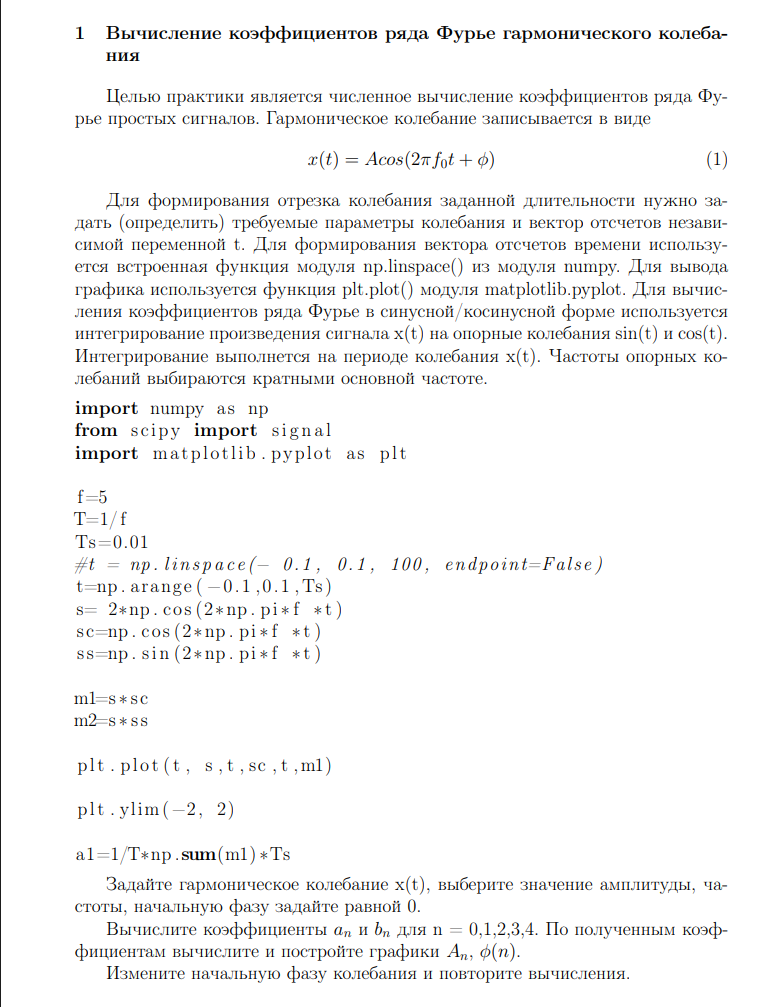
\includegraphics[width=1.0\textwidth]{tasks1.png}
    \caption{Задачи на практику}
\end{figure}

\begin{figure}[ht]
    \centering
    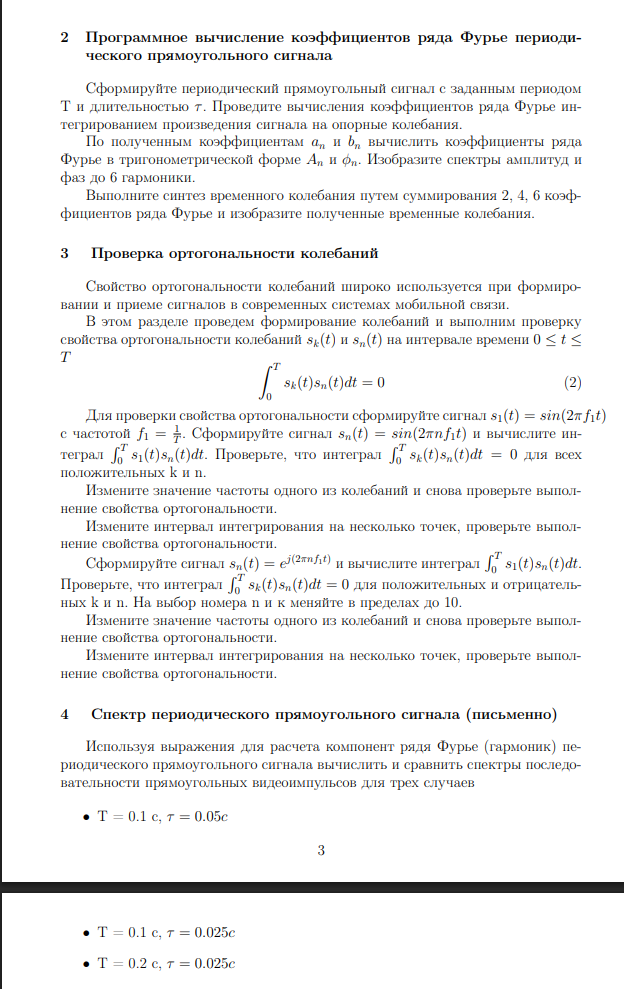
\includegraphics[width=1.0\textwidth]{tasks2.png}
    \caption{Задачи на практику}
\end{figure}

\endinput